\documentclass[a4paper, 11pt]{article}

%\usepackage[parfill]{parskip}
\usepackage{ragged2e}
\usepackage{graphicx}
\graphicspath{ {images/} }
\usepackage[T1]{fontenc}

\newlength{\drop}
\usepackage{epigraph}
\usepackage{dirtytalk}
\usepackage{wrapfig}
\usepackage{quoting}
\usepackage{courier}
%\usepackage{titlesec}
\usepackage{tabularx} 
\usepackage{pbox}

%\setcounter{secnumdepth}{4}

%\usepackage[pdftex,active,tightpage]{preview} 
%\setlength\PreviewBorder{2mm} 
\usepackage{gantt}
\renewcommand{\epigraphflush}{center}
\renewcommand{\epigraphwidth}{1\textwidth}

%........................
% Header/Footers
%........................
\usepackage{lastpage}
\usepackage{fancyhdr}

%%%%%%%START%%%%%%%
\begin{document}
  \begin{titlepage}
	\thispagestyle{empty}
    \drop=0.1\textheight
    \centering
    \vspace*{\baselineskip}
    \rule{\textwidth}{1.6pt}\vspace*{-\baselineskip}\vspace*{2pt}
    \rule{\textwidth}{0.4pt}\\[\baselineskip]
    {\Large{MSc Computer Science\\[0.3\baselineskip] }} 	
    {\huge{Project Report\\[0.3\baselineskip] }}
	
    \rule{\textwidth}{0.4pt}\vspace*{-\baselineskip}\vspace{3.2pt}
    \rule{\textwidth}{1.6pt}
    \\[\baselineskip]
    \scshape
    {\Large Ubiquitous Consumer Inventory Management System For Waste Prevention\\}
%    Location, date from--to\par
    \vspace*{2\baselineskip}
    %Edited by \\[\baselineskip]
    {\normalsize\emph{Supervisor: }{\large Professor George Roussos\par}}
    {\normalsize\emph{Author: }{\large Keimi Okamoto\par}}
    
    {\itshape 2015}
    \vfill
    {\large BIRKBECK UNIVERSITY OF LONDON\par}
{\footnotesize DEPARTMENT OF COMPUTER SCIENCE \& INFORMATION SYSTEMS}\par
  \end{titlepage}
  
%\maketitle

%........................
% Contents
%.......................
\pagenumbering{roman}
\tableofcontents
\clearpage

\clearpage



%........................
% Introduction
%........................

\pagestyle{fancy}
\renewcommand{\sectionmark}[1]{\markboth{#1}{}}
\fancyhf{} % sets both header and footer to nothing
\renewcommand{\headrulewidth}{0pt}
\setlength{\footskip}{80pt}
\lhead{}
\chead{}
\rhead{Project Report}
\pagenumbering{arabic}
\lfoot{Section \thesection}
\cfoot{\fancyplain{}{\leftmark }} 
\rfoot{\thepage\ of \pageref{LastPage}}

\setcounter{page}{1}
\section{Introduction}

\subsection{Abstract}
What the project is about in regards to the proposal. The problem i am trying to solve. Over production food.
Tackeling the core, If the consumers stop over purchasing the supermarkets will stop over producing. 


\subsection{Structure of the report}
Present the reader with an overview of each chapter.

\subsection{Development Methodology}
UML and agile. And the reasons why this is a productive methodology.
Version control for documentation and history. 
\clearpage

%..................................................
% Background
%..................................................
\section{Background \& Analysis}
The first section of this chapter presents the problem and the motivation for the project. Then an analysis of currently available processes that are implemented to tackle the problem will be discussed. The last section will provide an analysis of the technologies that will aid the development of the system leading to the design of the application. 

\subsection{Motivation}

\subsubsection{Environment}
Globally, food waste has exceeded to two billion tonnes annually. This excessive generation of waste has a severe impact on our environment. Spoiling foods emit methane, a particularly harmful greenhouse gas contributing to the warming of the earth's surface and causing the expansion of the hole in the earths ozone layer. The ozone layer is vital to the survival of living organisms as it protects against harmful radiation form the sun. Too much exposure can result to illnesses such as cancer and eye damage. 

Resources used during the rearing and plantation process for produce as well as the manufacturing materials for packaging and fuel used for transportation all contribute to the detrimental effect on our environment. Councils are continuously pressured to fuel more funds into waste management recourses and landfill sites are overflowing at such a rapid pace space to accommodate the waste is fast diminishing.

In the United Kingdom alone consumers and households are responsible for at least seven million tonnes of waste, whilst in comparison the retailers contribute a mere two hundred and twenty five thousand tonnes. Although the reported figures implicate the household as the primary culprit, retailers are in fact the catalyst force behind the mass generation of waste. Competition for market share is fierce between the retailers and goods must always be available at a lower price than that of their neighbours. Frequent buy-one-get-one-free and multi-buy discounts hosted by retailers contribute largely to the problem. Farmers and other producers alike are pressured to over produce to accommodate for the probability of a sudden rise in demand or to simply cover the risk of a potentially bad harvest. But when the sales forecast is not met or the harvest is overly fruitful, supermarkets will routinely deduct the price of food nearing expiration as a method of damage control for their investment. Consumers are enticed by the attractive offer of a free item after purchasing two, and encouraged to over purchase food that they do not need and will most likely not consume before the use-by-date. Thus, waste that was originally created by the retailers is pushed down the chain and ultimately residing with the consumers. This aggressive sales strategy not only causes monetary waste to the consumer but also engineers the blind participation in driving up demands in goods, in turn encouraging the overproduction of food. 


\subsubsection{Public Health}
In addition to the environmental damage, there are growing concerns over public health risks the bargains offers bring. Over purchasing of food can encourage excessive consumption. Discounted foods usually come with a shorter use-by-date, meaning over a shorter span of time an individual must consume more than necessary in order for their investment to be justified. This side effect is detrimental to the health and well being of the public as the national statistics report for the United Kingdom has unveiled. Obesity rates in male adults have increased 13.2\% and 7.4\% for female adults since 1993. These figures are rising every year and the World Health Organisation (WHO) has predicted that by 2030 74\% of male adults and 64\% of female adults will be obese if precautionary measures are not implemented. 

\subsubsection{Aiding the Modern Lifestyle}
The final problem is simply human errors. We purchase produce with the good intention of consuming them. But as the demands of our fast paced modern life-style take priority, we often forget all about the existence of what we stocked and inadvertently let our stock expire. Expiry dates for products vary, and keeping track of them all is a near impossible task by relying on human memory alone. A popular study carried out in by George Armitage Miller, a prominent figure in the field of cognitive psychology discovered that the number of objects an average human can hold in working memory is seven, give or take two. With this limited capacity it is no surprise that once the fridge door is closed, it is inevitable that some of the produce is destined for the waste bin.

Additionally many homes are made up of multiple inhabitants. Errors such as double purchasing due to lack of communication is a common occurrence. If two occupiers notice an item is low on stock at different times they may both set out to replace the item, resulting in duplicate items being purchased and increasing the risk of waste occurring. 


\vspace{\baselineskip}
\vspace{\baselineskip}
\subsection{Current Waste Reduction Methods}
Governments and organisations have taken various measures to tackle the rising figures in waste. Below describe the techniques used and the strengths and weaknesses that each possess. 

\subsubsection{Manual Labour} 
Governments have launched Campaigns aimed to educate the public on the implications of waste. The registered charity, part funded by the government, Waste \& Resources Action Programme (WRAP) have frequently interacted with communities by setting up stalls and public demonstrations to raise awareness. This form of engagement is inspirational and informative but also a very expensive operation and sustaining the interest of the community is difficult and effects are short lived.%\cite{2}

\subsubsection{Anaerobic Digestion} 
Waste management organisation Biffa and the retail giant Sainsbury's have collaborated in an effort to convert waste into energy by recycling food waste using a method called anaerobic digestion. By utilising the gases produced from the decomposing food they are able to generate power which in turn is used to sustain the running of retail stores. Anaerobic digestion creates a circular process where the waste produced by the retailers is pumped back into the production line to fuel the very instrument creating the problem. This method has been questioned as to whether it is a true solution to the problem as the resources used throughout the process also leave a carbon footprint.\cite{anarobicDigestion}



\subsubsection{Smart Fridge} Smart fridges were introduced in the early 2000's as a home inventory management system. Designed to be integrated into our every day lives and to monitor the inhabitants inventory. The user inputs product details on an embedded screen or mobile device. Some are equipped with barcode scanners as another method of registration. The fridge was designed to monitor inventory and to inform the owner if items are running low on stock. If the fridge detected that inventory was running low an order would automatically made to the retailer. The primary drawback of this product is the cost of the appliance and lack of infrastructure supporting an efficient product registration proccess. With one unit costing over \$20,000 and items still dependant on manual registration or time consuming barcode scanning many were discouraged

\subsubsection{Nano Technology} 
Most recently Nano technology has been used to monitor the stages of decomposition in foods. A small gel like cube emits a colour corresponding to a particular stage of decomposition and visually representing the shelf life of the product. Nano technology is able to remove the need for printed sell-by-dates but it still requires the inhabitants to actively open the fridge door, view, process and memorise the colours of the tags for various products. 

\subsubsection{Mobile Application} 
Existing waste management applications include the self titled application by 'Love Food Hate Waste' (LFHW). The application include features such as a shopping lists memo maker, recipe suggestions, portion size suggestions. The Netherlands Nutrition Centre Foundation (NNCF) funded by the Dutch government, have released an app `Smart Cooking' that incorporates similar features to LFHW. TooSkee and LeanPath\cite{FoodWaste} are other examples of food management apps developed by organisations in the United States. Much like the other apps it will suggest dishes and remind the user to consume products before the expiration date. 

But these product logging applications suffer from the same bottleneck, the act of having to manually punch in the product details or scan each barcode with a reader. This arduous process dissuades many users and can result in the application being discarded. 


\subsubsection{Radio Frequency Identification} 
NXP Semiconductors, a Dutch research team have collaborated with the Netherlands Packaging Centre (NPC),  to develop a sensor enabled RFID tag capable of monitoring the environmental changes though the supply chain. \cite{rfidFood} The Pasteur sensor tag has the capacity of measuring shifts in temperature and gas conditions during transportation and various stages of storage. An accurate prediction of the product's shelf life is generated from the data collected, enabling prioritisation of the trading of supplies, reducing the likelihood of waste. At the currents state this is only available for large-scale shipments to suppliers from the producers.

\subsection{Item Level Identification}
The primary draw back of existing systems such as the smart fridge and the mobile applications is the lack of automation in the item registration process. Convincing consumers to alter habitual behaviours such as stocking the fridge is challenging and would most likely be met with resistance unless the new process yields better results than the current. Thus, the user having to either manually punch in the product name, or scan every item with a barcode reader is an unappealing process and can prevent the user from utilising the technology. 

\subsubsection{Current Item Level Product Identification Methods} 
Predominantly, the current methods of item level identification in the supply chain rely on the "picket-fence" style, one-dimensional barcodes \cite{add image Barcodes} have been prevalent in grocery stores since the 1970's and introduced as a means to manage inventory and to accelerate the checkout process. A laser scans the code and the catalogued code is used to retrieve details of the item, such as the name and cost. The scanning of the barcode requires that no objects obstruct the line of sight between the code and laser and even the smallest scratch or dirt can render the code unreadable. Simultaneous reads are not possible and codes must be scanned one by one with precision. Barcodes also have limited capacity; usually can only hold twenty to twenty-five characters. Furthermore, the code is limited to identifying a collection of items rather than the individual item level, omitting crucial fine-grain information such as sell-by-dates and the life-cycle of produce. 

\subsection{Proposed Approach to the Problem}
In attempts to reduce the generation of food waste, the British government has intervened and officials pressured retailers to abolish the multi-buy offers. But the suggestion was met with reluctance. Instead a compromise was reached and the revised promotions allowing consumers a wider variety of products to choose from. Although figures declined periodically it was not maintained. It is evident from this that persuading retailers to prioritise the reduction of waste over the increase in revenue is an up hill struggle. Without constant monitoring, retailers will favour the increase in revenue over the betterment of the public. 

For this reason the proposed solution is not to persuade the retailer to change their practice but the consumer. By equipping the consumer with an application that is able to monitor their inventory overstocking can be discouraged. The consumer will be driven by the incentive of monetary savings and as a side-effect reduce the risk of waste occurring at the consumer level. Theoretically creating an upstream ripple effect that will keep the waste at bay with the retailers and forcing the termination of over production. 

\subsubsection{Proposed System}
The proposed system is comprised of two key components. The first is the RFID client and the second an Android application. For the RFID application a RFID reader will reside in the fridge, monitoring the presence of any tags in its vicinity and facilitating the automatic registration when loading and unloading products from the fridge. The system will keep an accurate inventory of the users contents and communicate any changes to the user's smartphone.

\subsubsection{Mobile Applications}
As popularity in smartphones increase many applications have identified the need for ubiquitously accessible counterpart software. Whether it is in the form of a web applications, such as the popular taxi booking application Uber or by using available mobile platforms such as IOS for Apple or Android, the way in which we utilise software has shifted from the traditional static machines to mobile systems. The convenient size and connectivity has enabled Smart devices to evolve rapidly and daily tasks such as checking emails can now be completed on the move. With many applications with similar functionalities available with a tap of a screen and with a market place where a single bad review can jeopardise the success of an app, quality and functionality is paramount, users have become increasingly intolerant of a poor interface design or performance such as delayed content loading. 


\subsubsection{Cloud Services} %%%%%%%%%%%%%%%%%%%%%
%%%%%%%%%%%%%%%%%%%
%%%%%%%%%%%%%%%%%%%%

\subsubsection{Item Level Product Identification Using RFID} 
RFID utilises electromagnetic waves emitted by a reader. The tag is comprised of a coil and transistor that harvests the energy from the reader. Once the tag has enough power, the data is transmitted and the information may be read from the tag. 

NFC registration and stock keeping systems have been successfully installed in retail stores, in particular clothing retailers. Before, logging of stock was a manual task. Employees would walk around the store floor with a laser reader and scan each item one by one. If the barcode had been damaged they would have to note the reference number down to enter into the system at a later time. With the use of RFID the employee now holds a reader and walks by the rack of garments, where the tags are read simultaneously, and the details captured with ease. Some grocery stores also use NFC but the technology is reserved for valuable goods to serve as an anti-theft device. Tags are applied in the form of a sticker and when detected by the readers, normally situated at the store exits, it will trigger an alarm to notify staff.

NFC has a few advantages over the traditional method of product identification. Firstly the tag does not require a clear line of sight. The reader may interrogate any tag within the vicinity of the transmitted electromagnetic field. The energy is passable through objects and some readers can even facilitate simultaneous reads. Secondly, tags are more durable than the traditional printed kind and can be embedded within the packaging or inconspicuously applied to the product. NFC also has more space to hold data.

With the use of RFID the consumer need not alter any behaviour. The item registration process can be completely automated removing the need for the consumer to manually enter product information or line-up lasers with barcodes. Some other benefits can also be experienced through the application of item-level RFID. 



\subsection{Case Studies to Support the Use of RFID at the Item-Level}

\subsubsection{Transparency \& Consumer Rights} The need for transparency of the origin of the produce is important to better the quality of living. Granular information can help consumers control what they consume to aid a healthier life. Produce information is often documented by the producers and passed to the supplier but the information fails to make it down the chain.[18] Meats in particular have unique backgrounds. Ranging from the rearing environments, type of feed consumed and drugs administered. This information can provide awareness to consumers whether it is for health reasons, environmental or the ethically conscious individual. 
Such areas as Japan where vegetables and livestock were exposed to nuclear radiation due to the Fukushima Daiichi disaster raises serious health concerns. Damage caused by radiation exposure by consumption of contaminated foods can surface much later in a persons life and in some cases even be inherited by offspring. This highlights the urgency for transparent detail of the product?s life cycle and the importance for the consumer to be fully aware of the risks and responsible for what they consume.[20] 
The law enforces that the label on fresh meat must contain the country of origin. But this does not apply to the same meat that is processed, such as hamburgers, pies and sausages. Meats may be mixed providing that the animals are slaughtered in the same country, meaning a single hamburger could be made up of several cows.[18] Officials have used over crowding of labels as a reason not to provide the customer with details of a produce and has deemed it unnecessary. 
?It is clear that many consumers want more information on the origin of meat ingredients in meat products, and in the Agency?s consumer research the ingredients in dairy produce also score highly in this respect. The law requires an origin declaration on fresh beef but not on the same product when it has been seasoned. Providing information on the origin of all ingredients in all products would be disproportionately burdensome for industry, and would risk overload- ing the label with information that is not seen as important by consumers.?- Food Standard Agency, ?country of origin labelling guidance?[18] 
With the use of RFID the overloading of the label would no longer be a reason to withhold information from the consumer. Allowing the individual to decide what information is of importance. 

\subsubsection{Food Safety \& Tractability} In the past there has been numerous incidents when products have been recalled due to the presence of bacteria or other abnormalities. A notable incident is the 2013 meat adulteration scandal in the EU, where traces of horse meat where dis- covered in various products such as minced meat and ready prepared meals. The time and resources to trace back through the supply chain was estimated to have cost the Food Standard Agency (FSA) \pounds900,000 between 2011 and 2012 and a further �1.6 million between 2012 and 2013 [18]. Other casualties include the reputations and integrity of the blameless producers falsely accused due to limited and inaccurate information that implicated them as the guilty.[9] 
With item level identification the contaminated produce could be traced back immediately and the products recalled.[13][14] For example if an infected animal is used in various products, all items holding that particular code can be instantly traceable, effectively compartmentalising the outbreak and maximising efficiency in damage control. 

\subsubsection{Remote Amendment of Human Errors} Frequently food is wasted due to human errors. On the 13th April 2015, a mass recall for 'Starbucks Black \& White Mini Cookies' was issued due to undeclared use of milk products. Misprinting of information or neglecting to provide adequate product details that abides by the food standard regulations are a common error in the production pipeline and perfectly consumable food is wasted. By applying RFID tags to groceries products, errors can be amended remotely and immediate alerts issued, notifying customers of the mistake. This provides a different approach to error management and can avoid the generation of unnecessary waste. 

\subsubsection{Efficient Checkout Process} The traditional checkout process requires the cashier to scan each item one by one, even with the new self checkout systems introduced to reduce queuing time, the line is often held up by an unreadable barcode or the numerous failed attempts of the laser initiating a read. Items must be loaded out of the basket or shopping-trolley and places into a shopping bag. As demonstrated by MyGrocer, a system that was designed to modernise the shopping experience, utilises a trolley lined with RFID readers. As tagged products are loaded the readers record the presence of goods and upon checkout all the user needs to do is pay a bill. 

\subsubsection{Discounting Tags} When products are nearing expiration it is common practice for the retailers to discount the products. A store assistant will usually carry a barcode-printing device that generates a sticker with the discounted code. He or she will manually check the date and if the item is eligible a sticker with a new discounted barcode will replace the original. With the use of RFID the amendment can be made remotely and automatically, filtering and amending only the relevant products. 

\subsection{Technology Risk Analysis}
\subsubsection{Mobile Platforms}
Currently the most popular mobile platforms are Android and Apple IOS. Android currently has the largest user base, boasting an estimate of one billion users. IOS applications are written in languages such as Objective C, which require the developer to manage the memory of objects. Recently, a new language Swift was introduced by Apple. Swift supports automatic reference counting (ARC), this eliminates large memory leaks that frequently occurred in it's predecessor Objective C. Android on the other hand has a high-performance memory management system that cleans up unused objects, also know as the garbage collector. This feature allows the developer to focus their time and attention on the functionality of the application. Android applications are written in Oracle Java. It is also note worthy to mention that Android has a unique ecosystem unlike that of a typical Java application. The developer must understand and abide by the rules of the environment, failing to do so can result in undesired outcomes. 

Swift being a relatively young language means that less support is available compared to the others, increasing the risks of encountering difficulties. Objective C will require diligent memory management and can shift focus from the core of the application development and problems may arise from the lack of personal expertise. Having previous exposure to Java, as it was taught as a core module (Programming in Java), the Android development environment was a sensible option. The familiarity of the language and integrated memory management feature minimised the risk of encountering difficulties. Android also has a larger user base making the application accessible to a wider audience.

\subsubsection{Cloud Services} 
Cloud services have gained notoriety due to the I.T giants Google, Amazon and Microsoft. The underlining principals of cloud computing of automated scalability and constant availability of resources have converted the way I.T businesses operate. Enabling small organisations to begin developing with minimal capital expenditure. Traditional in house server farms require thousands of pounds for initial setup, but by delegating the responsibility of upgrades, maintenance and load balancing to a cloud vendor, focus can be kept on developing the application. To further emphasis, more businesses are adopting the agile methodology where change is to be expected and must be embraced\cite{}, cloud services facilitates change by only charging the user for the resources consumed, in effect renting the software and hardware, giving teams agility to react to change with minimal financial risk.

Utility bill style billing and the ability to the respond to peaks and troughs of demand are ideal for this project. Much like most online retailers where for the most part experience steady traffic, but during the holiday seasons and sale periods could potentially experience a sudden peak when consumers are most active. In the past the unpredictable nature of human activity has resulted in server crashes but with the use of a cloud service the system can scale seamlessly.

Out of the three leading cloud service Google Cloud Platform (GCP), Amazon Web Services (AWS) and Microsoft Azure the most fitting is AWS. Azure is recommended for those who are currently utilising the Microsoft stack such as C\# and MySql neither of which is relevant for this project. GAE's data analytics engine has been praised as superior to that of AWS owed to the massive amounts of data harvested by Google.\cite But in terms of services available AWS is without a doubt the leading vendor (see image).  AWS also has higher availability with eleven geographical locations that resources can be distributed to and users anywhere can efficiently access, in comparison Google has only three regions. Although a notable disadvantage with AWS's myriad of services is grasping the understanding of the complex network topology, this creating a steeper learning curve than GCP. Although GCP is simpler and user friendly it has been concluded that the positive elements of AWS has outweighed the negative.

\subsubsection{RFID Technology}
There are many different classifications of RFID readers and tags that differ in the amount of memory it can hold to the range and direction it may transmit data. Radio waves transmitted by the readers differ in frequency from low (LF) to high (HF) to ultra-high frequency (UHF). LF readers typically operate at 125KHz with a read range of around 10cm, as the frequency increased the read range also expands and so may the sensitivity to radio wave interference. 

Tags also vary in specifications, passive tags may only be activated by a reader and may not instigate a transaction, where as semi-active and active tags may start communications. For this project the focus will be Near Field Communication(NFC). NFC is most notably used in transport ticketing and contactless payment management systems. NFC has successfully automated the ticketing and payment systems in many countries. Instead of manually punching in digits on a keypad, the user can touch or wave the NFC embedded card near the reader and a transaction can be processed. RFID has sped up various registration and transaction processes. NFC is inexpensive and durable, making it a primary candidate for tagging on mass produced food products that are frequently moved from different containers during the transportation process. Many mobile phones currently available on the market also are equipped with NFC readers further supporting the argument for the utilisation of NFC.

\subsubsection{Data Storage Method}
For any system the way in which data is stored and received strongly impacts system performance. Relational database management systems (RDBMS) provide a secure, reliable, tried and tested method of data management. Data is organised into schemas that are designed using normalisation techniques and queried using structured query language (SQL). Schemas are predefined and RDBMS comply with the ACID properties. 

Although RDBMS provide a robust and secure data management solution, in some cases it's not the best solution. A common problem with RDBMS is the relationship ambiguity that the schemas can present even after the data is normalised. For example, the image below, one might argue that that it is describing one person with two qualifications but another may interpret this as two separate entities which happen to have the same name but with different degrees. Schemas are predefined and constraints are applied to disallow invalid values. One way in which RDBMS ensures consistency is with the utilisation of strict locking protocols but heavy locking of tables and rows can case threads to wait and compromises availability to ensure consistency of data. 

%%% add image 


The inability to articulate how the data is to be perceived and the need for BigData processing on massively distributed systems was a motivational factor for the NoSQL movement. NoSQL databases are flexible and schema-less, many compromise consistency with availability and operate on the principal of eventual consistency. NoSQL databases can vary from document, graph and key value storage methods. Data can be modelled dynamically and entities are in charge of their own attributes.

For this project high availability of the recourse takes precedence over consistency. Flexibility is needed when modelling the data as the system may need to respond to change rapidly, thus, a NoSQL data storage solution is fitting for the solution. 

\subsubsection{Distributed Authentication \& Access Control}
Different security levels and access restrictions must be enforced depending on the user to avoid data corruption and data breach. For cloud services in particular, where each account is billed on a pay-as-you go basis, if resources and credential are not regulated appropriately the account owner can amass in an unexpectedly large bill. AWS SDK provides an access control service that can be implemented using an API. Different roles and policies may be assigned to users, granting granular level permissions. 

\clearpage

%..................................................
% Design
%..................................................
\section{Design}
The first part of this section will present the system requirements and use cases for the application. The second part will discuss the design decisions driven by the analysis of technologies and existing systems made in the previous chapter.

\subsection{Requirements}
Information gathered in the analysis stage has highlighted the following requirements. Requirements will help identify the core functionality of the application and 

\subsubsection{Automated Product Logging Using RFID}
The logging of products must be automated using RFID technology. The RFID interrogator is to be embedded in a fridge were it must listen for incoming and outgoing tagged products. The logging mechanism must provide accurate real-time stock keeping of products.
 
\subsubsection{Offline Inventory Management}
The RFID application must have a local cache that logs items even when an Internet connection is not present. When connection resumes the cache and the database must be consistent. 

\subsubsection{User Verification}
Users must be verified from an Android device in order to use the service. Authentication must be made possible either by email or a popular third-party user authentication API. By keeping a record of the users if the user happens to remove the application and later decide to reinstall the application. The previous account can be restored allowing the user to skip time-consuming registration steps. User verification is also a necessity to avoid the wastage of cloud recourses.

%%%%%%%%%%%%%%%%%%%%%%%DONE UP UP UP
%%%%%%%%%%%%%%%%%%%%%%%DONE UP UP UP
%%%%%%%%%%%%%%%%%%%%%%%DONE UP UP UP
\subsubsection{Access Control to Resources}
The RFID client and Android client must have different layers of access to resources. AWS credentials must not be hard coded into applications as the application is intended for mass distribution across multiple devices.

\subsubsection{Data Organisation}
Data must be available via wireless communication and must be constantly available to facilitate the displaying of real-time representation of the users inventory. Data must be organised and follow best practice data modelling techniques. 

\subsubsection{Multiple user support}
A single fridge may have multiple users. Application use must mirror real life scenarios where multiple users exist for one fridge. Once a user is verified via the Android application he or she will have the opportunity to enter a unique fridge code that will grant them access to view the contents of the fridge. 

\subsubsection{Displaying Fridge Contents}
The contents must be visible on an Android powered Smartphone. When connected to the Internet the data should be consistent with the current state of the fridge. Items will display the products in priority order with the earliest use-by-date at the head and the latest at the tail. 

\subsubsection{Offline Content Viewing}
For situations where there is no Internet connection or sudden loss of connection the last view of the fridge before the connection is terminated must be visible. To enable this feature a local cache must be made that saves the intermediate data.

\subsubsection{Engaging Users with Notifications}
When a new item is added to the fridge it must push a notification to all android devices subscribing to a particular fridge.  Ensuring all parties is up to date with the alterations. 

\subsubsection{User Interface}
The user interface must be easy to navigate and follow Android best practices. Instantly recognizable icons and screen gestures will be utilised to ensure the user has a stress free introduction to the application.

\subsection{Requirements Definition Report}
A requirement definition report is provided to support the development of the new system. Here the requirements are organised into categories following the UML recommended presentation as described in the book, ?System Analysis and Design with UML? by Tegarden and Wixom. (Suggestion was taken from the Information Systems module as part of the MSc Computer Science.)

\subsubsection{Non-Functional Requirements}
\underline{Operational Requirements}
\begin{itemize}
  \item The mobile element system should be able to operate in an Android environment. 
  \item The system should be portable and accessible from a mobile phone.
  \item The system should persist and read data from the database. 
  \item The system should scan and register RFID tags.
\end{itemize}
\underline{Performance Requirements}
\begin{itemize}
  \item The user interface must constantly be active.
  \item The system should be available for use 24 hours per day, 365 days per year.
  \item Any communication between the clients and the server must not exceed 5 seconds.
  \item The system should be durable and preserve data integrity.
\end{itemize}
\underline{Security Requirements}
\begin{itemize}
  \item Only authorised users can use the system.
  \item Users may only see the content of the subscribed fridge.
\end{itemize}

\vspace{\baselineskip}

\subsubsection{Functional Requirements}
\underline{Multi-user Support}
\begin{itemize}
  \item Any user should be able to join an existing fridge by entering the unique code provided to the primary owner of the fridge.
\end{itemize}
\underline{Information Viewing}
\begin{itemize}
  \item User should be able to view a list of their stocked items.
  \item User should be able to view the expiry date of the items with ease. 
  \item User should be able to see the quantity for each item.
  \item User should be notified when an item is added to their inventory.
  \item Users may only see the content of the subscribed fridge.
\end{itemize}
\underline{User Registration}
\begin{itemize}
  \item Users should be able to login to the system. 
  \item User should be able to logout by pressing the logout button.
\end{itemize}


\subsection{Use Case Reports}

\subsubsection{User Login}
\begin{center}
\noindent\resizebox{\textwidth}{!}{
\begin{tabular}{ | l | l | }
 \hline
 \textbf{Use Case} & Initial start up of Android Application.   \\ 
 \hline
 \textbf{Primary Actor} & A member of the public who installs the application.  \\ 
 \hline 
 \textbf{Description} & \pbox{10cm}{A ew user opens the application for the first time.} \\ \hline 
  \textbf{Assumptions} & \pbox{10cm}{1.The application is installed and running on a device running the Android environment. \\2. The device is connected to a wireless Internet connection.\\3. The RFID client is successfully running.} \\
  \hline 
 \textbf{Success Scenario} & \pbox{10cm}{ 1. A user selects the application icon on the home screen. \\2. The application does not recognise the user as previously registered and will display the login page.\\3. The user will enter valid credentials and grant permissions for the application to access user information.\\4. The user will then be directed to a page to enter a unique Fridge code. The user will enter a valid code.\\5.The user will succesfully subscribe to the and will be presented with the contents of the fridge in order of priority with the latest expiary date at the top.} \\ 
 \hline 
  \textbf{Alternative Flows} &  \pbox{10cm}{If the user has previously signed up the sign up process is skipped and the user is presented with the main page.\\ If the user does not have and valid credentials they will not be able to proceed.} \\  \hline 
 \textbf{\pbox{4cm}{Non-Behavioural \\Requirements}}&  \pbox{10cm}{User details must be stored in the database. Only users with a valid fridge ID is able to access the contents of a particular fridge.} \\ 
 \hline 
 \textbf{Issues} &  n/a\\ 
 \hline 
\end{tabular}
}
\end{center}






\subsubsection{Add item into the fridge.}
\begin{center}
\noindent\resizebox{\textwidth}{!}{
\begin{tabular}{ | l | l | }
 \hline
 \textbf{Use Case} & User loads the fridge with items.\\ 
 \hline
 \textbf{Primary Actor} & A member of the public who installs the application.  \\ 
 \hline 
 \textbf{Description} & \pbox{10cm}{A user who has a RFID embedded fridge stocks the fridge with tagged items.} \\ \hline 
  \textbf{Assumptions} & \pbox{10cm}{1.The application is installed and successfully running in a Java runtime environment.\\2. The component is connected to the Internet.\\3.The fridge's unique code persists in the database.\\4.All items that are loaded into the fridge are tagged with RFID tags.} \\
  \hline 
 \textbf{Success Scenario} & \pbox{10cm}{ 1. A user opens the fridge and adds the products.\\2.The tag is registered and interrogated for it's ID.\\3.The item ID is stored in the user's database.\\ 4. When an item is removed the RFID reader will read and the application ID will be removed.} \\ 
 \hline 
 \textbf{Alternative Flows} & \pbox{10cm}{If Internet is not present the item ID is persisted locally.} \\ 
 \hline 
 \textbf{\pbox{4cm}{Non-Behavioural \\Requirements}}&  \pbox{10cm}{If there is no Internet connection the application must save the tag ID's locally. Once the connection is present the data must be saved to the database.} \\ 
 \hline 
 \textbf{Issues} &  n/a\\ 
 \hline 
\end{tabular}
}
\end{center}




\subsubsection{Refresh Contents.}
\begin{center}
\noindent\resizebox{\textwidth}{!}{
\begin{tabular}{ | l | l | }
 \hline
 \textbf{Use Case} & User can refresh content view upon request.\\ 
 \hline
 \textbf{Primary Actor} & A member of the public who installs the application.  \\
 \hline 
 \textbf{Description} & \pbox{10cm}{Using the pull down gesture the contents of the fridge can be refreshed and displayed.} \\
  \hline 
 \textbf{Assumptions} & \pbox{10cm}{1.The application is installed and running on a device running the Android environment. \\2. The device is connected to a wireless Internet connection.\\3. The RFID client is successfully running.\\4.The user has successfully signed in.} \\
  \hline 
 \textbf{Success Scenario} & \pbox{10cm}{ 1. User pulls the list down and releases. 2. If any changes have occurred in the fridge the list will be updated displaying the latest informattion. } \\ 
 \hline 
 \textbf{Alternative Flows} &  \pbox{10cm}{n/a} \\ 
 \hline 
 \textbf{\pbox{4cm}{Non-Behavioural \\Requirements}}&  \pbox{10cm}{The application must display data as close to real time as possible. Any alterations to the database will trigger a notification to the user.} \\ 
 \hline 
 \textbf{Issues} &  n/a\\ 
 \hline 
\end{tabular}
}
\end{center}


%%%%%%%%%%%%%%%%%%%%% USER LOGOUT USE CASE %%%%%%%%%%%%%%%%%

\subsection{Business Process Modelling with Activity Diagrams}
\subsubsection{User Login}
Figure \ref{fig:LoginActivity}

\begin{figure}[p]
\centering
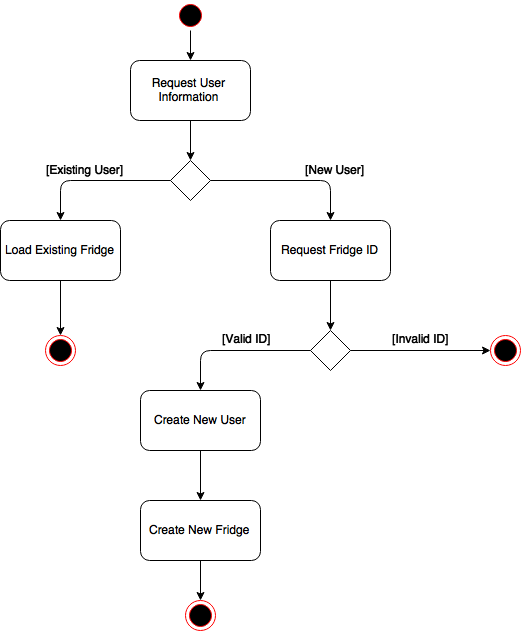
\includegraphics[width=\textwidth]{LoginActivity}
\caption{Activity Diagram for the user login flow.} \label{fig:LoginActivity}
\end{figure}

\subsection{Program Design}
This section defines the programs that need to be written and the methods that will be utilised to satisfy the requirements.

\subsubsection{Distributed Authentication \& Access Control}
The authentication process will be completed through the Android application. One AWS account may be used for multiple applications and so it is important to authenticate users and only grant access to the relevant resources. AWS Cognito and Identity and Access Management (IAM) tool kit provides an API and console to mange users and delegate role policies to restrict resource access. 

\subsubsection {User Authentication}
A user must be authenticated to avoid unnecessary AWS resource consumption. Authentication is to be made possible via email or a third-party service such as Facebook, Google or Twitter. Majority of users will have previously signed up to popular social networking sites and it has become a popular authentication pattern to utilise these services rather than to provide a custom sign up flow. By utilising existing API?s repetitive user behaviour can me avoided and provides a speedy hassle free process. 

\begin{figure}[h]
\centering
\includegraphics[width=\textwidth]{cognitoFlow}
\caption{Activity Diagram for the user login flow.} \label{fig:cognitoFlow}
\end{figure}

\subsubsection {Delay Tolerant Networking}
The system must be able to keep a consistent state by utilising a local cache on both the Android device and the Fridge application even in an event where Internet connection does not exist. Heterogeneous networks with multiple dependencies and the reliance on wireless Internet access must be fault tolerant

\subsubsection {Database \& File Specification}
\paragraph{AWS DynamoDB}Data will be stored in Amazon?s key-value NoSQL database DynamoDB. DynamoDB is a managed distributed database built on Solid State Drives (SSD) for efficient low latency response time. Data is free to store and Amazon will only charge for throughput used. As user demand grows DynamoDB is able to scale seamlessly and traffic is managed and balanced automatically. The highly available nature is backed by a robust fault recovery mechanism. Data is replicated across multiple nodes to ensure that even in a situation where a cluster is damaged and is offline another is always available. 

\paragraph{Internal Device Storage}The Android application will utilise the devices internal storage to localise retrieved data.  The SharedPreference class is a lightweight method of storing data in a key-value pair. For complex objects on both the Android application and RFID application the Java I/O library will be used to serialise data.  

\subsubsection {Interface Design}
Over the years Smartphone users have become accustom to certain navigation patterns. Keeping with popular gestures and icon designs provides the user with a stress free user experience. For example users instinctively recognise certain icons to give a particular functionality such as the ?settings? button. (See image below). It would be ineffective to redesign a settings icon and make the user learn a new pattern of navigation and can even cause the user to reject the application. A common pattern for refreshing a list is to pull down the screen where a loading icon is displayed. This feature is to be implemented for refreshing the screen. The interface must constantly be responsive and provide feedback to the user to avoid the user thinking the application has crashed. 

\subsubsection {RFID Client}
The RFID client will be written using the Java development kit version 8, using the IntelliJ Integrated development Environment (IDE). The AWS SDK will also be used to access DynamoDB resources. Tag ID?s will be read and persisted in the relevant fridge where the android application will receive the data. The hardware will be connected to an Internet enabled computer with the Java Runtime Environment installed. A console will display a log to communicate any errors that may occur. 

\begin{figure}[p]
\centering
\includegraphics[width=\textwidth]{RFIDApplicationFlow}
\caption{Activity Diagram for the user login flow.} \label{fig:RFIDApplicationFlow}
\end{figure}

\subsubsection {Android Client}
The Android application will be written using Java and utilise the Android SDK version 4.4 to target as many devices as possible. The application will be developed using Android Studio IDE and the AWS Mobile SDK. Implementation will take into consideration Android?s unique activity lifecycle methods to avoid undesired behaviour. Android development and object oriented best practices will be applied to maximise code reusability and minimise decoupling of classed to avoid strong dependencies between classes and activities.

\clearpage

%...................................................
% Implementation
%..................................................
\section{Implementation}

\subsection{RFID Java Client Development}
\subsubsection{Hardware}The selected interrogator is a 125khz Mifare technology RFID reader. It has a short read range of up to ten centimetres. The tag type is an ISO/IEC 14443 standard, passive low frequency RFID embedded stickers.

\subsubsection{Application} 
The java client continuously polls for incoming tags. When a tag is read the unique code is extracted and queried against the database. Once the item is successfully identified the product is added to the users table. Where the Android client may retrieve the data, thus automating the item registration process. When the same item is read the reader will acknowledge the removal of the item and the product is removed from the table.
In the even of a network failure a local cache will store the item ID?s, details on the implementation can be found in the section -----Delay Tolerant Networking. 

\subsection{Android Development} 

\subsubsection{Android Activity \& Life Cycle Methods}
Android uses a component called an activity to depict an action a user may accomplish within the application. When an activity class is extended some key methods listed below may be overridden and custom behaviour can be implemented. The developer has no control over when the methods are called and so given a situation the implementations can vary. Figure \ref{fig:activity} shows the life cycle of an activity and the methods that may be called. Careful management and implantation of the methods is needed to avoid unexpected behaviour and system crashes.

Activities may be launched as an intent. When activities are launched they are places on top of a stack, where the history of the activity is kept, this is called the back stack. Upon the user pressing the back button the current activity is popped off the stack and they may return to the previously running activity. 


\subsubsection{Login Activity}
The login activity is responsible for the user authentication process. Graphical elements such as buttons and text boxes instantly translate the needed actions the user is to take. 

**Add image

\paragraph{Buttons}
The LoginActivity class implements the \texttt{onClickListenter()} interface which enforces the implementation of the \texttt{onClick()} method. In this method a switch statement is used to determine which button was pressed. The switch statement checks for the interacted resource ID and executed the necessary block . For example, \texttt{R.id.facebook\_login\_button} corresponds to the Facebook login button. 

When the Facebook button is pressed the  user must go through Facebook?s authentication process if the user has not previously signed up. If the user is a retuning user then the login process is avoided and the user is directed straight to the main activity.  

When the user enters their credentials, a request for an access token is made to Facebook. If the user is a registered member of Facebook a new activity is launched requesting that the user grant the application permission to extract the listed details from their account. In this case the user?s profile and email address is needed to use the application, as shown in Figure \ref{fig:fbProfileEmail}. If the user accepts, a graph JSON object is retuned containing the user?s details and the next activity is launched.

\begin{figure}[h]
\centering
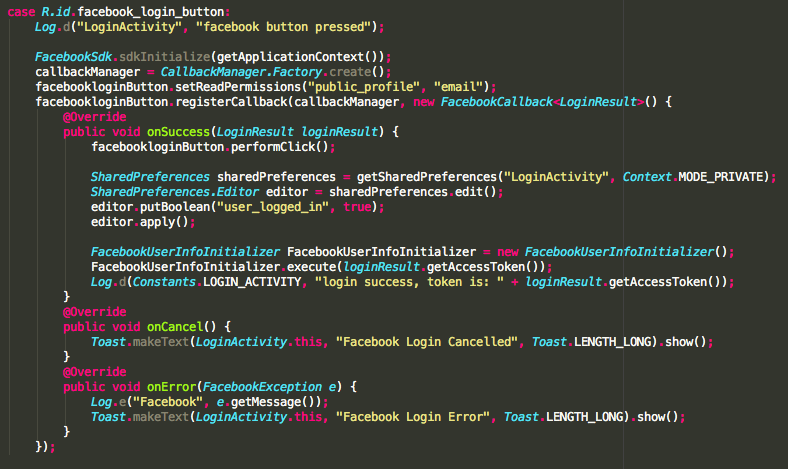
\includegraphics[width=\textwidth]{fbProfileEmail}
\caption{onClick() method implementation.}
\end{figure}

If the user is invalid the error will display a toast message communicating the failure to the user. The user will stay on the login page and will not be able progress until valid credentials are provided. 

Once the user has been authenticated this state is preserved to avoid the user needing to go through the signup flow each time the application is closed. Only when the logout button situated in the settings is explicitly pressed the user is logged out and in order for the user to use the app the sign up activity is launched again. 


\paragraph{Back Stack Management}
When launching a new Intent, flags may be added to it to manage the Back Stack. The history of the login page is not needed and does not need to be kept on the stack, doing so could even pose a security risk if the user is able to navigate back to the page where they entered confidential information. Also if the Back Stack is not managed, a trail of activities become visible when exiting the application and is perceived as bad practice and unprofessional. Activities that the user will never return to should be disposed of and should avoid being kept on the Back Stack. To ensure that the user cannot return to the login activity the history must be removed. By calling the Intents \texttt{addFlags()} method and passing it the parameters \texttt{Intent.FLAG\_ACTIVITY\_NO\_HISTORY}, if this is set then the intent is not saved in the tasks history.


\paragraph{Graceful Application shutdown}
Commonly, if the user is on the main page and the back button is pressed the application will exit and return to either the device home screen or the previously running application on the Back Stack. But as the aim is to get the user to sign up, if the back button is pressed the application will ask for confirmation from the user that the user truly would like to exit, if so the user is prompted to press the back button again. This is achieved by overriding the \texttt{onBackPressed()}method. 

**add image


\subsubsection{Fridge Code Request Activity}
Users will be able to subscribe to a fridge using this activity. The activity displays a text box there they are prompted to enter a unique ID. If the ID is valid the contents of the fridge will be retrieved and displayed. If the user is an existing user of the application this activity will not be launched and they will be directed to the main activity, listing the contents of their subscribed fridge.

After the user logs in the first a query will be made to the database to check if the user has previously signed up. If the records exist they are received and the EnterFridgeIDActivity is never launched. If no records exist this intent will be launched and the user will not be able to proceed unless the 

\paragraph{User actions and feedback}
When the application requires the user to input or edit a field the actions must be visually translated to the user. If no feedback is provided to the user they may mistake that the application has frozen or is broken. Toast messages may be used to provide feedback to the user. Here when an empty field is submitted the user will be prompted of their error. However if the entered id is invalid another message will be displayed so the user is informed of the mistake with accurate detail. 

**Add images both toast messages

\subsubsection{Main Activity}
The main activity is launched after the user is successfully authenticated. This activity will allow the user to remotely access the contents of the fridge. Below describes the construction process of the activity. 

\paragraph{Fragments} The Main Activity is made up of fragments. In Android development the use of fragments is encouraged to avoid duplication of code and to create a transportable UI element that can be used with devices that vary in screen size. Fragments can be composed into activates allowing UI elements to be transported with ease and promote code reusability. Fragments belong inside an activity and also has a life cycle of it?s own, similar to an Activity. The fragment can be declared in two ways. Either statically using the activities layout file, or programmatically set in the \texttt{onCreate()} method.  	

\paragraph{Custom List Adapter} 
As the format the data is presented in the list element is not available using the Android library, a custom list view and adapter were made. The \texttt{InventoryListAdapter} class extends an \texttt{ArrayAdapter}. The adapter class is responsible for dynamically setting the graphical elements and text fields in the list elements. 

 In the \texttt {onCreateView()} method in the \texttt{InventoryFragment} the custom adapter is set to the list view. As the activity?s \texttt{onCreate()} method is called and in turn the fragments are launched the information will display to the viewer. 

The \texttt{compare()} method in the products class is overridden and in the Adapter, the products are rearranged in priority order. The text will be displayed in red if the product is expiring today and green if there is no urgency. 

** Image 

\paragraph{Settings} 
The settings icon and location have conformed to the Android recommended design practice. As shown in \ref{fig:settings} the settings contains the logout button where the user must navigate to in order to logout. To implement this the ::onOptionsItemSelected() must be overridden. Same as the onClickListener() method it uses the resource ID to find which field was selected. 
 
\subsubsection{Graphical User Interface Design \& Resources}
Interface elements can be created using XML elements that make up the UI. Elements that build the GUI are declared inside the layout files and can be styled within the XML document. Alternatively graphical elements can be set at runtime programmatically using Views and ViewGroups objects, where graphical elements can be extracted and edited within the code. 

For each Activity and Fragment the application will style the interface using XML to keep the business logic and GUI logic separated, allowing the code to be more readable and maintainable. Figure \ref{fig:xml} is the layout used for the Main Activity. 

**image goes here

Resources such as graphical icons, logos, colours and Strings are stored in the values file within the resources. Strings are kept in a separate XML document so others may reference it and avoid hardcoding into the code and created a single access point where modifications can be made. Android operates world wide so this approach can also facilitate the 

\subsubsection{Manifest File}
All Android application has a manifest file. Activities, services, receivers and content providers must all be registered in this file in order for them to be utilised. Permission are also set here to enable privileged features such as access to the Internet and cross application data sharing. Application name and screen orientation and even setting the start up activity is declared in this document.

\subsubsection{Notifications}
Android uses notification alerts to communicate with the user. Notifications can be triggered when certain events occur. When a new item is added to the fridge an alert is triggered notifying the user of the change in state. This way even without the user having the application open they are kept informed of the state reducing the likelihood of the user unknowingly purchasing the same product.

**add image
\subsubsection{Threads \& Concurrency Management}
\subsubsection{Service and BroadcastReceiver 
\texttt{ScheduleReceiver}
}


\subsubsection{Error Handling}
\paragraph{Exceptions}
\paragraph{Logging}


\subsection{Distributed Authentication and Access Control}

Access control to resources is imperative to avoid security breeches and data loss. When using AWS mobile SDK, AWS enforces the use of Cognito for mobile identity management. Cognito uses Identity Pools to manage the different layers of user privileges and Identity Access Management (IAM) roles.

\subsubsection{Identity Pool}
An identity pool is specific to the application. As a single AWS account is used by many different applications the segmentation of users can help organise the subscribing users and facilitate the allocation of correct recourses to the user. 

By using the Cognito client developers can avoid hardcoding credentials into the application?s source code. This is particularly important for programs intended for mass distribution. 

The image below is a method that initialises the Cognito client using the activities context, Identity pool id of the Amazon Resource Name (ARN) and the region code the resource resides on, in this case it accessing the servers in Ireland.  
%\vspace{\baselineskip}

\begin{figure}[h]
\centering
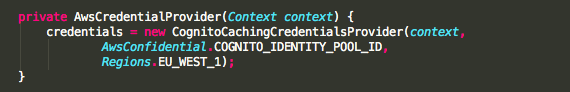
\includegraphics[width=\textwidth]{cognito_client_code.png}
\caption{Initialisation of Cognito Client}
\end{figure}

\subsubsection{Identity Access Management Role}
IAM Roles are assigned in identity pools. IAM roles allow fine grain access control to AWS resources such as S3 and DynamoDB. The Cognito client utilises the IAM role?s ARN to specify the access rights of each role. By default AWS creates an authenticated and unauthenticated access role for an identity pool. Authenticated users may only access the specified resources in the policy if the requirements are met in the statement. Unauthenticated roles are for users that may want to try the application before committing to signing up. Internally, temporary credentials are created for an unauthenticated user granting them temporary access to resources. 

\begin{figure}[t]
\centering
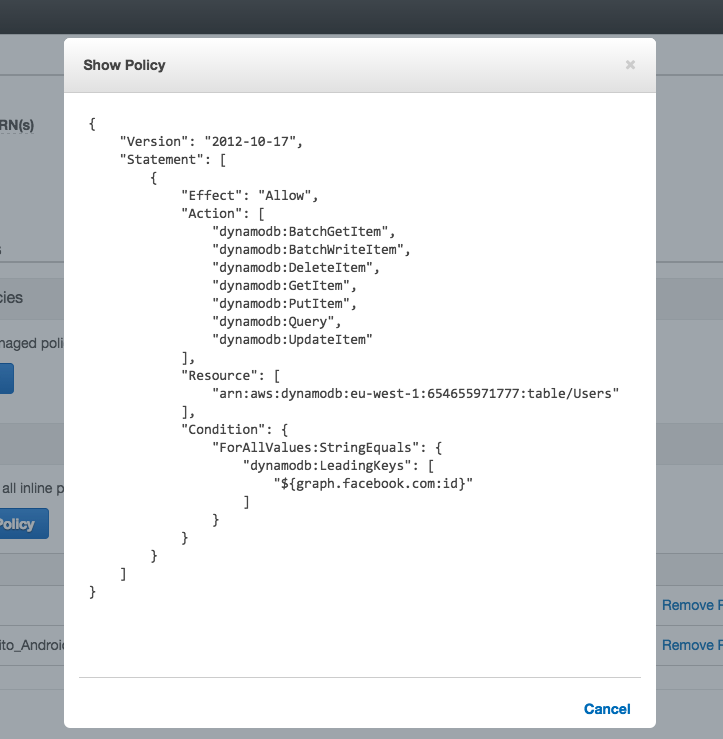
\includegraphics[width=\textwidth]{iam_policy.png}
\caption{Policy for Authenticated Users}\label{fig:iam}
\end{figure}

\paragraph{Security Policy}Policy statements are written in Java Script Object Notation (JSON). The statement is split into three sections, actions, resource and effect. The action block specifies the actions that are allowed on the service. For example the policy in Figure \ref{fig:iam} lists the actions that may be performed on a service, in this case DynamoDB. Actions that are not explicitly specified will be rejected. Resource block specify the AWS recourse that the policy is allowing access to, a resources is indicated by the ARN. The effect block specifies the result after the user requests access to the service. By default the effect is set to ?deny? so this must explicitly set. Additionally, a condition block may be set to further restrict the type of user gaining access. In the example below only users associated with Facebook are granted access.

\subsection{Delay Tolerant Networking}
\subsubsection{Caching}
%-Analytics, how these api's provide analytics, user patterns

\subsection{Data Management}

\subsubsection{Data Modelling}
\paragraph{Primary Key \& Range}
The primary key consists of a hash value. DynamoDB uses this unique attribute to identify items in the table. Additionally a range key may also be defined when creating the table. //What does the range key do

\paragraph{Secondary Index}


\subsubsection{Querying Tables}
Once the connection is established using the Cognito client the DynamoDB client can be initialised using the returned credentials. Classes that are intended to be persisted in the tables must be decorated with DynamoDB anotations. The annotated classes are translated into JSON format and added to the specified table. By placing \texttt{\@DynamoDBTable(table Name="Fridge")} before the class declaration the object can be utilised by DymanoDB. The primary key field is also required to be notated with \texttt{@DynamoDBHashKey}. Any other field that DynamoDB would like to interact with must also be annotated with \texttt{DynamoDBAttribute}. Similarly range keys and secondary indexes are also needed. Using the object mapper data can be stored and retrieved with ease. Figure --- shows an implementation of the Products class and an example query.

\subsubsection{Android Storage}

\clearpage


%...................................................
% Testing and evaluation
%..................................................
\section{Testing and Evaluation}
Importance, maintainable code.
\subsection{Unit Tests \& Mocking}
\subsection{Integration Test}

%...................................................
% Conclusion 
%..................................................
\section{Review and Conclusion}
\subsection{Security Concerns} look at link from George. 

%cite
%Case study re title to the researched products



\vspace{\baselineskip}
\vspace{\baselineskip}
\vspace{\baselineskip}


\end{document}
